%%%%%%%%%%%%%%%%%%%%%%%%%%%%%%%%%%%%%%%%%%%%%%%%%%%%%%%%%%%
%% Supporting Information
%%
%%%%%%%%%%%%%%%%%%%%%%%%%%%%%%%%%%%%%%%%%%%%%%%%%%%%%%%%%%%



% %%%%%%%%%%%%%%%%%%%%%%%%%%%%%%%%%%%%%%%%%%%%%%%%%%%%%%%%%
\subsection{Density functional theory (DFT) computational details}
% %%%%%%%%%%%%%%%%%%%%%%%%%%%%%%%%%%%%%%%%%%%%%%%%%%%%%%%%%
%
% %%%%%%%%%%%%%%%%%%%%%%%%%%%%%%%%%%%%%%%%%%%%%%%%%%%%%%%%%
% | - DFT Computational Details

% %%%%%%%%%%%%%%%%%%%%%%%%%%%%%%%%%%%%%%%%%%%%%%%%%%%%%%%%%
% | - General intro to shared DFT settings
% Things like the code used
% __|
% %%%%%%%%%%%%%%%%%%%%%%%%%%%%%%%%%%%%%%%%%%%%%%%%%%%%%%%%%
% | - PARAGRAPH BODY
%
Here we describe the density functional theory (DFT) methodology used for both the active learning bulk structure prototype optimization and the OER slab calculations.
%
The calculations were performed using DFT at the generalized gradient approximation (GGA) level of theory as implemented in the Vienna \latin{ab-initio} simulation package (VASP)~\cite{Kresse1995,Kresse1996_0,Kresse1996_1},
and utilizing the PBE exchange-correlation functional~\cite{Perdew1996}.
%
All calculations were performed with the inclusion of spin-polarization which is important for surface calculations of Ir-oxides~\cite{Briquet2017,Strickler2019} and utilized the projector-augmented wave pseudopotentials (PAW)~\cite{Blochl1994}.
%
Calculations were carried out through the atomic simulation environment (ASE) python interface.~\cite{HjorthLarsen2017}
%
% __|
%%%%%%%%%%%%%%%%%%%%%%%%%%%%%%%%%%%%%%%%%%%%%%%%%%%%%%%%%%%


% %%%%%%%%%%%%%%%%%%%%%%%%%%%%%%%%%%%%%%%%%%%%%%%%%%%%%%%%%
% | - Bulk DFT Specific Settings
%
% __|
% %%%%%%%%%%%%%%%%%%%%%%%%%%%%%%%%%%%%%%%%%%%%%%%%%%%%%%%%%
% | - PARAGRAPH BODY
Here we describe the DFT methodology and workflow for optimizing the candidate structures for the AL algorithm.
%
We employed a higher plane-wave cutoff of \SI{600}{\electronvolt} for bulk relaxation compared to OER slab calculations (\SI{500}{\electronvolt}).
%
A variable k-point mesh was used, with a k-point density of at least \num{20} k-points per \AA$^{-1}$ reciprocal space dimension.
%
All bulk systems were run through the following computational recipe to converge the equilibrium structure, with \num{3} distinct phases. Structures are only advanced to the next phase when the previous phase completes without error.

\begin{enumerate}
  % %%%%%%%%%%%%%%%%%%%%%%%%%%%%%%%%%%%%%%%%%%%%%%%%%%%%%%%
  \item
  %
  A unit cell volume relaxation that constrains the relative values for the cell lattice parameters to keep the unit cell volume shape constant (ISIF 7).
  %
  This optimization is the coarsest and least susceptible for failure to account for initial geometries being far from physical and hard to converge.
  % %%%%%%%%%%%%%%%%%%%%%%%%%%%%%%%%%%%%%%%%%%%%%%%%%%%%%%%
  \item
  %
  A series of three successful bulk optimizations that relax all degrees of freedom (atom positions, cell shape, and cell volume),
  and corresponds to a ISIF \num{3} flag in VASP.
  %
  The reason we run three consecutive ISIF \num{3} runs is to ensure that the unit cell dimensions are unaffected by the well known basis errors associated with changing the unit cell size during optimization.
  % %%%%%%%%%%%%%%%%%%%%%%%%%%%%%%%%%%%%%%%%%%%%%%%%%%%%%%%
  \item
  %
  For good measure, a final optimization was performed keeping the unit cell constrained (ISIF \num{2}).
  %
  These energies typically differ by less than \SI{10}{\milli\electronvolt} compared to the previous ISIF 3 optimization.
  %
  This step employs a more stringent self-consistent field (SCF) energy convergence criteria of \SI{1e-6}{\electronvolt} and force convergence of \SI{1e-3}{\electronvolt\per\angstrom}
\end{enumerate}
% __|
%%%%%%%%%%%%%%%%%%%%%%%%%%%%%%%%%%%%%%%%%%%%%%%%%%%%%%%%%%%
% %%%%%%%%%%%%%%%%%%%%%%%%%%%%%%%%%%%%%%%%%%%%%%%%%%%%%%%%%
% | - OER Specific Settings
%
% __|
% %%%%%%%%%%%%%%%%%%%%%%%%%%%%%%%%%%%%%%%%%%%%%%%%%%%%%%%%%
% | - PARAGRAPH BODY
Here we briefly describe the DFT computational details for slab calculations.
%
For a more thorough description of the OER methodology, including surface energies and determination of OER activity refer to sections below.
%
A 4$\times$4$\times$1 k-point mesh with $\Gamma$-centered Monkhorst-pack mesh~\cite{Monkhorst1976} was used for all OER slabs.
%
All slab calculations maintained a vacuum spacing of approximately \SI{15}{\angstrom} on average.
%
Dipole corrections were imposed on all non-symmetric slabs to counteract the effects of density dipole interactions.~\cite{Neugebauer1992}
%
Roughly \num{3/4} of the bottom layers were kept fixed to simulate the bulk crystal while the top two surface layers were allowed to fully relax.
%
All structures were relaxed utilizing the conjugate gradient algorithm as implemented in VASP (IBRION\num{=2}).
%
The slab optimization was run until the maximum force on all atoms was below the force threshold of \SI{0.02}{\electronvolt\per\angstrom}.
% __|
%%%%%%%%%%%%%%%%%%%%%%%%%%%%%%%%%%%%%%%%%%%%%%%%%%%%%%%%%%%

% __|


% %%%%%%%%%%%%%%%%%%%%%%%%%%%%%%%%%%%%%%%%%%%%%%%%%%%%%%%%%
\subsection{Structural candidate generation methodology}
% %%%%%%%%%%%%%%%%%%%%%%%%%%%%%%%%%%%%%%%%%%%%%%%%%%%%%%%%%
%
% %%%%%%%%%%%%%%%%%%%%%%%%%%%%%%%%%%%%%%%%%%%%%%%%%%%%%%%%%
% | - Generation of Structural Candidates

% %%%%%%%%%%%%%%%%%%%%%%%%%%%%%%%%%%%%%%%%%%%%%%%%%%%%%%%%%
% | - Candidate Generation Intro
% Basic intro into candidate generation
% High-level overview again
%   * Data mining OQMD MP fro AB2/3 entries
%   * Reduce data set by eliminating structurally redundant systems
%     * This is done with Ankit's scheme
% __|
% %%%%%%%%%%%%%%%%%%%%%%%%%%%%%%%%%%%%%%%%%%%%%%%%%%%%%%%%%
% | - PARAGRAPH BODY
%
Here we describe the methodology to construct the set of structural candidates in more detail.
%
The first step of the procedure is to mine materials databases for entries with the desired non-element specific stoichiometry (\latin{i.e.} \ABtwo and \ABthree).
%
Since many of the entries in these databases are structurally redundant,
we used a structure classification scheme to reduce the data set to a structurally unique set.
%
Once this is accomplished, the elements of interest were then substituted into the database structures,
which at this point had their original elemental composition from their database entries.
%
Finally, the structures are isotropically expanded or contracted to accommodate the difference between the atomic radii of the original elements in the structure and the user defined elements.
%
This procedure of ``pre-optimization'' is an important step because
it is necessary to generate reasonable initial geometries which would otherwise produce poor fingerprint representations and lead to a large degree of structural drift during the course of DFT optimization.
% __|
%%%%%%%%%%%%%%%%%%%%%%%%%%%%%%%%%%%%%%%%%%%%%%%%%%%%%%%%%%%


% %%%%%%%%%%%%%%%%%%%%%%%%%%%%%%%%%%%%%%%%%%%%%%%%%%%%%%%%%
% | -
% Data-mining OQMD and MP
% __|
% %%%%%%%%%%%%%%%%%%%%%%%%%%%%%%%%%%%%%%%%%%%%%%%%%%%%%%%%%
% | - PARAGRAPH BODY
%Herein, we take advantage of the structural diversity already present in materials databases to construct our candidates.
%
We utilized two materials databases, the Open Quantum Materials (OQMD)\cite{Saal2013} and the Materials Project (MP) databases\cite{Jain2013} because of their large and diverse sets of crystalline inorganic materials.
%
% TODO Approx. when did Ankit parse these databases
At the time that we originally mined these databases (2018) there were \num{61471} inorganic compounds in the MP database and \num{435583} entries in the OQMD database.
%
We note that the databases have expanded the number of entries considerably since we originally parsed them,
but we don't expect that the number of unique structural prototypes has increased significantly.
% __|
%%%%%%%%%%%%%%%%%%%%%%%%%%%%%%%%%%%%%%%%%%%%%%%%%%%%%%%%%%%


% %%%%%%%%%%%%%%%%%%%%%%%%%%%%%%%%%%%%%%%%%%%%%%%%%%%%%%%%%
% | - Ankit's paragraph on details on structural classification scheme
%
% __|
% %%%%%%%%%%%%%%%%%%%%%%%%%%%%%%%%%%%%%%%%%%%%%%%%%%%%%%%%%
% | - PARAGRAPH BODY
%
The structural classification scheme of Jain \latin{et al.}~\cite{Jain2018} was used to assign the crystal prototype,
consisting of standardized space group and Wyckoff positions,
as well as the element-nonspecific stoichiometry of each structure (\num{497054} in total).
%
This prototype designation can serve as a structural fingerprint and has successfully been applied towards the prediction of formation energies of inorganic compounds~\cite{Jain2018}.
%
Structures belonging to the same crystallographic space group and having the same participating Wyckoff sites have identical crystal symmetry and are grouped together into what we refer to as a ``structure prototype''.
%
Each unique structure prototype will contribute one structure to the final candidate set, thereby eliminating structurally redundant systems.
%
%We identified unique structure types by grouping materials according to participating Wyckoff sites.
%
The Wyckoff sites of crystallographic space groups are a collection of fractional coordinates within the unit cell where atoms are allowed to sit in order to satisfy the symmetry of the underlying space group.
%
The space group and standard setting of a unit cell is identified, and atomic positions are mapped to Wyckoff sites using the openly available, crystal symmetry library Spglib~\cite{spglib}.
%
The Wyckoff sites are subsequently mapped to unique Wyckoff-pair combinations, to obtain a unique classification which is independent of crystal translation and rotation.
%
The related Wyckoff sites are found by looping through all allowed crystal symmetry operations of the crystal.
%We mapped all such related Wyckoff sites to the same structure-type by looping through all allowed crystal symmetry operations of the crystal.=
%
Further mathematical details of these operations are available in Jain \latin{et al.}~\cite{Jain2018}.
% __|
%%%%%%%%%%%%%%%%%%%%%%%%%%%%%%%%%%%%%%%%%%%%%%%%%%%%%%%%%%%


% %%%%%%%%%%%%%%%%%%%%%%%%%%%%%%%%%%%%%%%%%%%%%%%%%%%%%%%%%
% | -
%
% __|
% %%%%%%%%%%%%%%%%%%%%%%%%%%%%%%%%%%%%%%%%%%%%%%%%%%%%%%%%%
% | - PARAGRAPH BODY
%
Once the structural prototypes are classified,
we selected all entries with the desired stoichiometry of \ABtwo and \ABthree from MP and OQMD.
%
Materials Project (MP) has \num{2424} and \num{2341} \ABtwo and \ABthree entries, respectively,
and OQMD has \num{4736} and \num{28883} \ABtwo and \ABthree entries, respectively.
%
The reason that there are considerably more \ABthree compounds in OQMD is due to the extensive compositional permutation of binary alloys in a cubic \ABthree structure.
%
Within each stoichiometry, the structural classification was used to eliminate structurally redundant systems using the structural classification scheme above.
%
This process reduces the data set to \num{620} and \num{219} unique structures of \ABtwo and \ABthree for MP and \num{397} and \num{194} structurally unique \ABtwo and \ABthree OQMD entries.
%
Combining the MP and OQMD data sets ultimately results in a dataset of \num{697} \ABtwo and \num{259} \ABthree structurally unique candidates.
%
A table summary of the number of entries in MP and OQMD at each step is outlined in Table \ref{table:database_structures}.
% __|
%%%%%%%%%%%%%%%%%%%%%%%%%%%%%%%%%%%%%%%%%%%%%%%%%%%%%%%%%%%


% =========================================================
% TABLE ===================================================
% =========================================================
% | - Table | OQMD MP Structures
\begin{table}[!htb]

  \caption{\label{table:database_structures}
    %
    (a) Number of entries in the OQMD and MP materials databases for the \ABtwo and \ABthree stoichiometries.
    %
    (b) Final number of unique structural candidates for \ABtwo and \ABthree.
    }
  %
  % | - Subtable a
  \begin{subtable}{.5\linewidth}
  \centering
  \caption{}
  %
   %
    %
    \begin{tabular}{cccc}
    \textbf{}         & \textbf{}        & \multicolumn{2}{c}{\textbf{Entries}} \\
    \textbf{Database} & \textbf{Stoich.} & \textbf{Total}   & \textbf{Unique}   \\
    OQMD              &                  & 435,583          &                   \\
                      & \ABtwo           & 4,736            & 397               \\
                      & \ABthree         & 28,883           & 194               \\
    \hline
    MP                &                  & 61,471           &                   \\
                      & \ABtwo           & 2,424            & 620               \\
                      & \ABthree         & 2,341            & 219
    \end{tabular}
    %
   %
  %
  \end{subtable}
  % __|
  %
  %
  \newline
  \vspace*{0.8 cm}
  \newline
  %
  %
  % | - Subtable b
  \begin{subtable}{.5\linewidth}
  \centering
  \caption{}
  %
   %
    %
    \begin{tabular}{cc}
    \multicolumn{2}{c}{\textbf{Final Candidate Set}} \\
    \textbf{Stoich.}   & \textbf{Unique Structures}  \\
    \ABtwo             & 697                         \\
    \ABthree           & 259
    \end{tabular}
    %
   %
  %
  \end{subtable}
  % __|
  %
\end{table}
% __| =====================================================
% =========================================================

% __|


% %%%%%%%%%%%%%%%%%%%%%%%%%%%%%%%%%%%%%%%%%%%%%%%%%%%%%%%%%
\subsection{Structure featurization and feature engineering}
% %%%%%%%%%%%%%%%%%%%%%%%%%%%%%%%%%%%%%%%%%%%%%%%%%%%%%%%%%
%
% %%%%%%%%%%%%%%%%%%%%%%%%%%%%%%%%%%%%%%%%%%%%%%%%%%%%%%%%%
% | - Structure Featurization and Feature Engineering

% %%%%%%%%%%%%%%%%%%%%%%%%%%%%%%%%%%%%%%%%%%%%%%%%%%%%%%%%%
% | - Voronoi tesselation and feature reduction
%
% __|
% %%%%%%%%%%%%%%%%%%%%%%%%%%%%%%%%%%%%%%%%%%%%%%%%%%%%%%%%%
% | - PARAGRAPH BODY
The bulk crystal structures studied here,
both the pre-optimized structural candidates and the post-DFT optimized systems,
were converted into numerical fingerprint vectors via the Voronoi tessellation method developed by Ward et al.~\cite{Ward2017}
%
The method produces a \num{271} length fingerprint vector where the \num{271} features encode both for chemical and structural information by constructing quantities that convolute atomic properties with the Voronoi neighbor shells.
%
Since we are applying the AL algorithm to each composition individually,
many of the \num{271} features become redundant (no variance) and thus we were able to immediately reduce the dimensionality of our feature space to \num{101}.
% __|
%%%%%%%%%%%%%%%%%%%%%%%%%%%%%%%%%%%%%%%%%%%%%%%%%%%%%%%%%%%


% %%%%%%%%%%%%%%%%%%%%%%%%%%%%%%%%%%%%%%%%%%%%%%%%%%%%%%%%%
% | - Feature processing and standardization
%
% __|
% %%%%%%%%%%%%%%%%%%%%%%%%%%%%%%%%%%%%%%%%%%%%%%%%%%%%%%%%%
% | - PARAGRAPH BODY
With the number of features reduced, it is then necessary to further process the raw numerical fingerprints to make them amenable for regression and fitting.
%
This included removing highly skewed data points, removing 0-variance features, and normalizing each feature by centering about the mean (mean of 0) and dividing by the features standard deviation (standard deviation of 0).
%
We expect that most of the remaining features are not linearly independent,
so that not all remaining features are crucial to retain,
%
For this reason, we chose to employ an additional feature reduction step by performing a principle-component analysis (PCA).
%
This allowed us to reduce the number of features to \num{10} while still capturing 99\% of the total variance and minimizing the cross-validated (CV) prediction MAE (Figure \ref{fig:cv_anal}).
%
This step is also crucial in reducing the computational expense of running the Gaussian Process training procedure.
% __|
%%%%%%%%%%%%%%%%%%%%%%%%%%%%%%%%%%%%%%%%%%%%%%%%%%%%%%%%%%%

% __|


% =========================================================
% FIGURE ==================================================
% | - Figure | Cross-validation analysis ******************
\begin{figure*}[!htb]
\centering
\makebox[\textwidth][c]{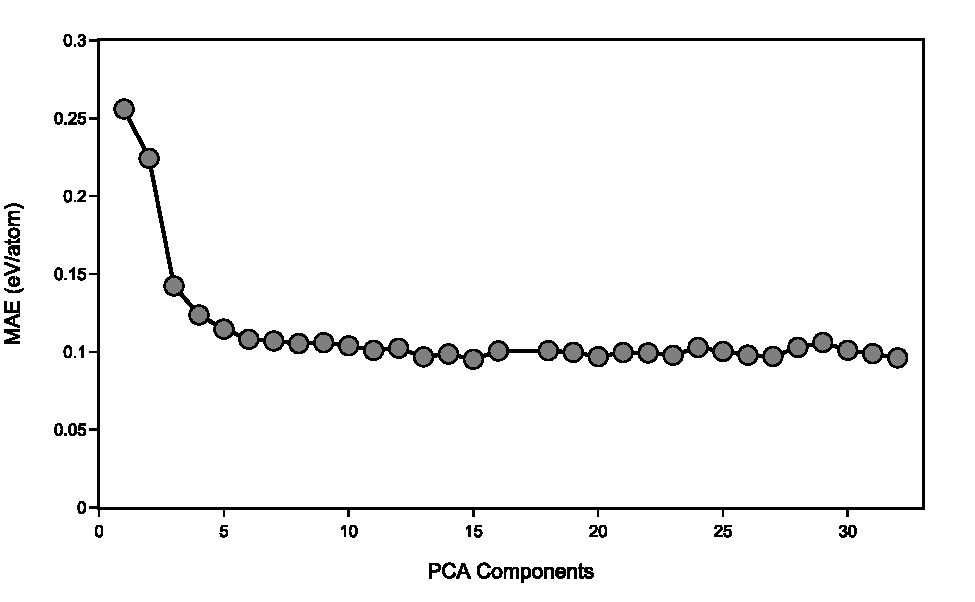
\includegraphics
{02_figures/SI_figures/00_mae_pca_plot__v0.pdf}}
\caption{\label{fig:cv_anal}
20-fold cross validation (CV) mean absolute error (MAE) as a function of the number of PCA components used for the GP-regression for \IrOthree.
%
Only post-relaxation fingerprints were used for both training and testing to avoid issues with structural drift.
%
All structural duplicates in the post-relaxation dataset were removed.
}
\end{figure*}
% __|
% =========================================================


% %%%%%%%%%%%%%%%%%%%%%%%%%%%%%%%%%%%%%%%%%%%%%%%%%%%%%%%%%
\subsection{Gaussian process regression and kernel selection}
% %%%%%%%%%%%%%%%%%%%%%%%%%%%%%%%%%%%%%%%%%%%%%%%%%%%%%%%%%
% Relevant details about the ML Gaussian process here
%
% %%%%%%%%%%%%%%%%%%%%%%%%%%%%%%%%%%%%%%%%%%%%%%%%%%%%%%%%%
% | - Gaussian Process Regression and Kernel Selection

% %%%%%%%%%%%%%%%%%%%%%%%%%%%%%%%%%%%%%%%%%%%%%%%%%%%%%%%%%
% | -
%
% __|
% %%%%%%%%%%%%%%%%%%%%%%%%%%%%%%%%%%%%%%%%%%%%%%%%%%%%%%%%%
% | - PARAGRAPH BODY
The active learning algorithm (AL) described here utilizes a regression model which can be trained on generated DFT data to predict the \DHf of unsampled candidates.
%
While almost any regression model would suffice, Gaussian process machine learning regression models were picked due to their highly flexible fits and high performance in situations with small data sets.
%
We utilized the Gaussian Process regression module as implemented in CatLearn.\cite{hansen2019atomistic,CatLearn_Repo}
%
The Gaussian Process recipe we developed utilized two isotropic Gaussian kernels which differ only in the values of the initial length scale parameter ($l$) and scaling parameter ($s$) (Eq. \ref{eq:gp_kernel}).
%
Here, isotropic refers to keeping the dimensionality of the kernel equal to one instead of an anisotropic kernel which was found to be difficult to with respects to optimizing the hyper-parameters.
%
The first GP kernel was constructed with a length scale parameter of \num{1} ($l_1$) and a scaling factor of 5 ($s_1$),
while for the second kernel the length scale and scaling factor were reduced by a factor of ten ($l_2$ and $s_2$).
%
This was done with the aim of producing a model that is responsive to both long- and short-range features in the input space.
%
Additionally, a regularization parameter ($\lambda$) which helps avoid over-fitting was set to an initial value of \num{0.025}.
%
% TODO Double check that I said it correctly, might be minimizing the LML
It should be stressed that these hyper-parameter values are only initial seed values, and that they will be optimized during every round of model training,
which occurs once per active learning loop,
and is done by maximizing the log marginal likelihood of the model and training data.
%
All hyper-parameter optimization is done internally in CatLearn.
% __|
%%%%%%%%%%%%%%%%%%%%%%%%%%%%%%%%%%%%%%%%%%%%%%%%%%%%%%%%%%%


\begin{equation}
    k(x,x') =
    s_1 exp \Bigl ( \frac{-|x-x'|^2}{2l_1^2}\Bigr) +
    s_2 exp\Bigl (\frac{-|x-x'|^2}{2l_2^2}\Bigr) +
    \lambda \delta_{x,x'}
    %
    \label{eq:gp_kernel}
\end{equation}


% __|




% %%%%%%%%%%%%%%%%%%%%%%%%%%%%%%%%%%%%%%%%%%%%%%%%%%%%%%%%%
% %%%%%%%%%%%%%%%%%%%%%%%%%%%%%%%%%%%%%%%%%%%%%%%%%%%%%%%%%
% %%%%%%%%%%%%%%%%%%%%%%%%%%%%%%%%%%%%%%%%%%%%%%%%%%%%%%%%%
% %%%%%%%%%%%%%%%%%%%%%%%%%%%%%%%%%%%%%%%%%%%%%%%%%%%%%%%%%
% %%%%%%%%%%%%%%%%%%%%%%%%%%%%%%%%%%%%%%%%%%%%%%%%%%%%%%%%%
% %%%%%%%%%%%%%%%%%%%%%%%%%%%%%%%%%%%%%%%%%%%%%%%%%%%%%%%%%
% %%%%%%%%%%%%%%%%%%%%%%%%%%%%%%%%%%%%%%%%%%%%%%%%%%%%%%%%%
% %%%%%%%%%%%%%%%%%%%%%%%%%%%%%%%%%%%%%%%%%%%%%%%%%%%%%%%%%




% %%%%%%%%%%%%%%%%%%%%%%%%%%%%%%%%%%%%%%%%%%%%%%%%%%%%%%%%%
\subsection{Active learning results for \IrOtwo}
% %%%%%%%%%%%%%%%%%%%%%%%%%%%%%%%%%%%%%%%%%%%%%%%%%%%%%%%%%
% Here are the analogous IrO2 results that were presented for IrO3 in the main text
% %%%%%%%%%%%%%%%%%%%%%%%%%%%%%%%%%%%%%%%%%%%%%%%%%%%%%%%%%
% | - Active Learning Results For \IrOtwo

% %%%%%%%%%%%%%%%%%%%%%%%%%%%%%%%%%%%%%%%%%%%%%%%%%%%%%%%%%
% | - Introduction Paragraph
%
% __|
% %%%%%%%%%%%%%%%%%%%%%%%%%%%%%%%%%%%%%%%%%%%%%%%%%%%%%%%%%
% | - PARAGRAPH BODY
%
Here we outline the results for the AL algorithm applied towards the space of all \IrOtwo candidates.
%
Interactive animations of the active learning algorithm for the runs shown in Figure \ref{fig:iro3_al} and \ref{fig:iro2_al} can be found as supplemental files titled
\texttt{AL\_IrO2\_Anim.html}
and
\texttt{AL\_IrO3\_Anim.html},
which can be opened in any web browser.
% __|
%%%%%%%%%%%%%%%%%%%%%%%%%%%%%%%%%%%%%%%%%%%%%%%%%%%%%%%%%%%


% %%%%%%%%%%%%%%%%%%%%%%%%%%%%%%%%%%%%%%%%%%%%%%%%%%%%%%%%%
% | - IrO2 AL General Results
% TODO Average number of runs to get R-IrO2
% TODO How many gens to obtain x/10
% TODO
% __|
% %%%%%%%%%%%%%%%%%%%%%%%%%%%%%%%%%%%%%%%%%%%%%%%%%%%%%%%%%
% | - PARAGRAPH BODY
%
Figure \ref{fig:iro2_al} shows the results of the active learning framework showcased here applied towards the space of \IrOtwo polymorphs.
%
The structure of Figure \ref{fig:iro2_al} is identical to Figure \ref{fig:iro3_al},
so the reader should refer to the main text for a more thorough explanation of all figure components.
%
In Figure \ref{fig:iro2_al}b six of the seven most stable \IrOtwo polymorphs are displayed.
%
The most stable phase corresponds to \rIrOtwo, the already established globally stable \IrOtwo polymorph,
which illustrates that our methodology can recover known phases readily.
%
Additionally, \rIrOtwo is quickly acquired by the AL algorithm,
with only \num{3.7} generations needed on average to pick rutile out of the candidates,
compared to 6.3 generations for the random acquisition.
%
This result is not totally surprising considering that \rIrOtwo is already present within the mined databases and so the initial candidate structure was already close to the final equilibrium geometry.
%
Additionally, our AL algorithm recovered other known phases of \IrOtwo, including columbite (\ref{fig:iro2_al}b.vi), pyrite (\ref{fig:iro2_al}b.vii), and anatase (not shown).
% __|
%%%%%%%%%%%%%%%%%%%%%%%%%%%%%%%%%%%%%%%%%%%%%%%%%%%%%%%%%%%


% %%%%%%%%%%%%%%%%%%%%%%%%%%%%%%%%%%%%%%%%%%%%%%%%%%%%%%%%%
% | - IrO2 AL Performance
%
% __|
% %%%%%%%%%%%%%%%%%%%%%%%%%%%%%%%%%%%%%%%%%%%%%%%%%%%%%%%%%
% | - PARAGRAPH BODY
Figure \ref{fig:iro2_al}c presents the discovery rate of the AL loop as a function of DFT bulk optimizations for the case of a GP-LCB acquisition criteria and the baseline random acquisition.
%
The results are qualitatively similar to the case of \IrOthree,
the GP-LCB method readily outperforms the random acquisition.
%
With only \num{200} DFT optimizations (\mytilde40\% of the entire candidate space) the algorithm discovered \num{9/10}ths of most stable systems,
while the random acquisition requires complete exhaustion of the candidates to find everything.
%
Interestingly the GP-LCB appears to saturate at nine structures, and is unable to find the tenth most stable structure until the candidate space is essentially exhausted.
%
Further investigation reveals that the hold-out structure has a very high predicted formation energy (\DHf),
despite the fact that it's post-DFT structure is the tenth most stable structure in dataset.
%
This result is another manifestation of structural drift between the pre- and post-optimized structures and indicates that the initial candidate structure was initialized in unreasonable coordinates and/or that the structure traversed a long distance through phase space such that the final and initial structures were no longer qualitatively similar.
%
This result highlights the importance of creating reasonable initial candidates.
% __|
%%%%%%%%%%%%%%%%%%%%%%%%%%%%%%%%%%%%%%%%%%%%%%%%%%%%%%%%%%%

% __|


% =========================================================
% FIGURE ==================================================
% =========================================================
% | - Figure | IrO2 Active Learning Results
\begin{figure*}[!htb]
\centering
\makebox[\textwidth][c]{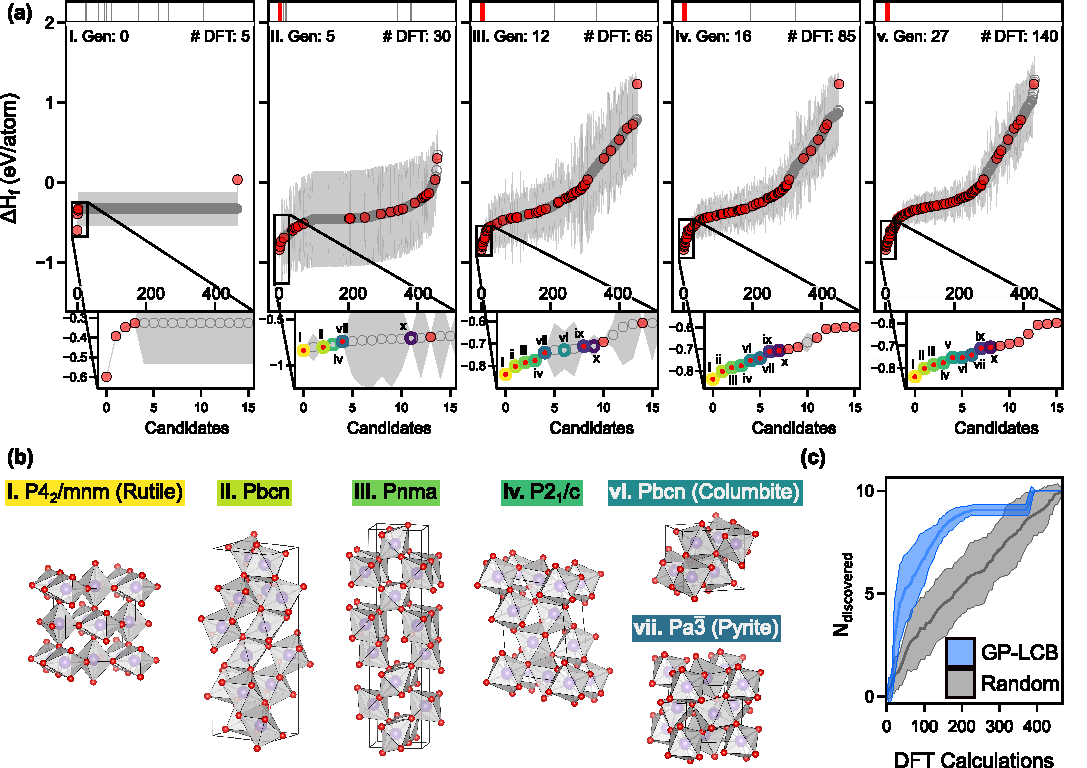
\includegraphics
{02_figures/SI_figures/00_ml_plot_iro2_al__v9__downsampled_1200x1200.pdf}}
\caption{\label{fig:iro2_al}
%
Results for the active learning algorithm applied to the \IrOtwo space.
%
This figure is analogous to Figure \ref{fig:iro3_al}, main text, which shows results for \IrOthree including the meaning of all symbols and labels.
}
\end{figure*}
% __| =====================================================
% =========================================================


% %%%%%%%%%%%%%%%%%%%%%%%%%%%%%%%%%%%%%%%%%%%%%%%%%%%%%%%%%
\subsection{Discovery rate for all active learning runs}
% %%%%%%%%%%%%%%%%%%%%%%%%%%%%%%%%%%%%%%%%%%%%%%%%%%%%%%%%%
%
% %%%%%%%%%%%%%%%%%%%%%%%%%%%%%%%%%%%%%%%%%%%%%%%%%%%%%%%%%
% | - Discovery rate of all runs of AL algorithms

% %%%%%%%%%%%%%%%%%%%%%%%%%%%%%%%%%%%%%%%%%%%%%%%%%%%%%%%%%
% | -
%
% __|
% %%%%%%%%%%%%%%%%%%%%%%%%%%%%%%%%%%%%%%%%%%%%%%%%%%%%%%%%%
% | - PARAGRAPH BODY
%
The entire AL algorithm was run a total of \num{100} times for both \IrOtwo and \IrOthree utilizing both the random and GP-LCB acquisition criteria (a total of \num{400} runs).
%
Each run was independent from the rest, with the only difference being the initial five candidates that were drawn to seed the algorithm.
%
Figures \ref{fig:iro3_al}c and \ref{fig:iro2_al}c show the results of the average discovery rate of these independent runs.
%
Figure \ref{fig:disc_rate} shows the same data, but with each individual run shown.
%
The red traces correspond to the specific runs that were plotted in Figures \ref{fig:iro3_al} and \ref{fig:iro2_al} and were chosen for being representative of the performance of the whole ensemble.
%
It is evident that the GP-LCB method has much less variability in its discovery rate compared to random, which is to say that it can more reliably acquire stable structures when compared to a random walk through the candidates.
% __|
%%%%%%%%%%%%%%%%%%%%%%%%%%%%%%%%%%%%%%%%%%%%%%%%%%%%%%%%%%%

% __|


% =========================================================
% FIGURE ==================================================
% =========================================================
% | - Figure | Discovery rate of all runs of AL algorithms
\begin{figure*}[!htb]
\centering
\makebox[\textwidth][c]{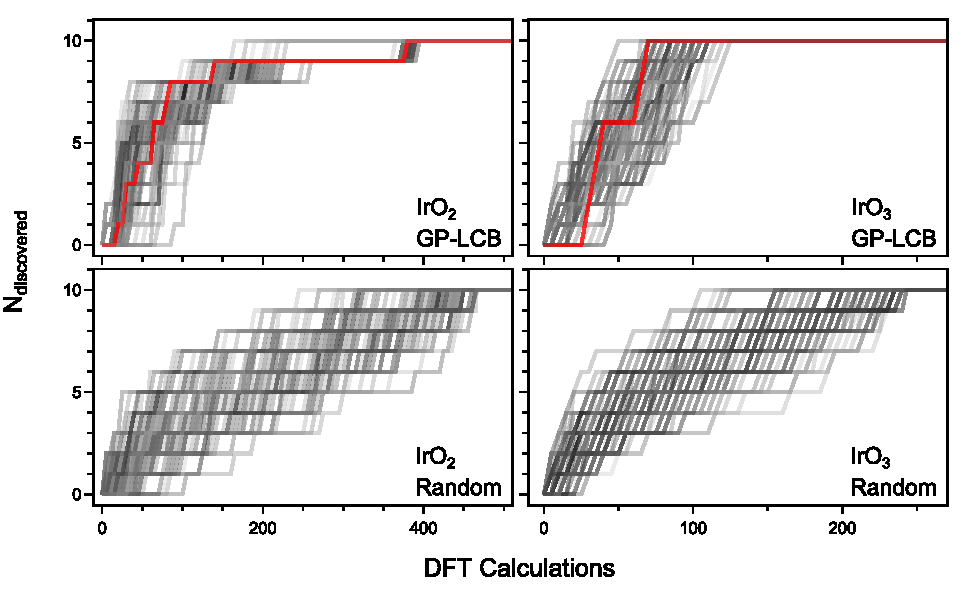
\includegraphics
{02_figures/SI_figures/00_disc_vs_dft__v2.pdf}}
\caption{\label{fig:disc_rate}
%
Quantity of top ten most stable \IrOtwo and \IrOthree polymorphs discovered ($N_{discovered}$) as a function of the number of DFT bulk optimizations performed for the GP-LCB acquisition and the baseline random acquisition methods.
%
Red lines indicate the specific runs used for Figures \ref{fig:iro3_al} and Figure \ref{fig:iro2_al}.
}
\end{figure*}
% __| =====================================================
% =========================================================


% % %%%%%%%%%%%%%%%%%%%%%%%%%%%%%%%%%%%%%%%%%%%%%%%%%%%%%%%%%
% \subsection{Structural Coordination Motif Analysis} %
% % %%%%%%%%%%%%%%%%%%%%%%%%%%%%%%%%%%%%%%%%%%%%%%%%%%%%%%%%%
% %
% % %%%%%%%%%%%%%%%%%%%%%%%%%%%%%%%%%%%%%%%%%%%%%%%%%%%%%%%%%
% % | - Structural Coordination Motif Analysis
%
%
% % %%%%%%%%%%%%%%%%%%%%%%%%%%%%%%%%%%%%%%%%%%%%%%%%%%%%%%%%%
% % | -
% %
% % __|
% % %%%%%%%%%%%%%%%%%%%%%%%%%%%%%%%%%%%%%%%%%%%%%%%%%%%%%%%%%
% % | - PARAGRAPH BODY
% TEMP section about doing the structural motif analysis. Maybe not needed.
% % __|
% %%%%%%%%%%%%%%%%%%%%%%%%%%%%%%%%%%%%%%%%%%%%%%%%%%%%%%%%%%%
%
%
% % __|


% %%%%%%%%%%%%%%%%%%%%%%%%%%%%%%%%%%%%%%%%%%%%%%%%%%%%%%%%%
\subsection{Amorphous limit as a thermodynamic upper bound for synthesizability of Ir-O polymorphs}
% %%%%%%%%%%%%%%%%%%%%%%%%%%%%%%%%%%%%%%%%%%%%%%%%%%%%%%%%%
%
% %%%%%%%%%%%%%%%%%%%%%%%%%%%%%%%%%%%%%%%%%%%%%%%%%%%%%%%%%
% | - Amorphous limit

% %%%%%%%%%%%%%%%%%%%%%%%%%%%%%%%%%%%%%%%%%%%%%%%%%%%%%%%%%
% | -
%
% __|
% %%%%%%%%%%%%%%%%%%%%%%%%%%%%%%%%%%%%%%%%%%%%%%%%%%%%%%%%%
% | - PARAGRAPH BODY
%
To provide a physically motivated energy cut-off for the potential synthesizability of the polymorphs we identify, we employed the procedure from Aykol et al. for determining the thermodynamic amorphous limit.~\cite{Aykol2018}
%
In this method, several amorphous configurations are sampled to find a relatively low energy configuration to use as a reasonable approximation to the amorphous limit.
%
We followed the computational procedure used by Aykol et al. to generate such sample amorphous phases for \IrOtwo and \IrOthree
(each amorphous phase comprising around 100 atoms),
and obtained 0.51 eV/atom and 0.31 eV/atom, respectively
(See Table \ref{table:amorph_limit}) for total and formation energies of sampled configurations).
%
It should be stressed that amorphous limits provide an stringent energetic upper bound for the synthesis of a crystalline polymorph at a given composition (i.e. polymorphs above the limit are inaccessible),
but they do not imply that polymorphs below the limits are necessarily physically realizable.
%
To expand, a crystal structure below the amorphous limit may still be kinetically inaccessible or simply restructure into another more stable configuration.
%
As such, being below the amorphous limit is a necessary but insufficient condition for a polymorph to be synthesizable.
% __|
%%%%%%%%%%%%%%%%%%%%%%%%%%%%%%%%%%%%%%%%%%%%%%%%%%%%%%%%%%%

% __|


% =========================================================
% TABLE ===================================================
% =========================================================
% | - Table | Amorphous Limit Data
\begin{table}
\centering
\caption{\label{table:amorph_limit}
%
Density functional theory computed energetics of sampled amorphous phases for \IrOtwo and \IrOthree as per the procedure of Aykol \latin{et al}~\cite{Aykol2018}.
%
Here we report the raw DFT electronic energy per atom ($E_{DFT}$),
the enthalpy of formation (\DHf),
and the energy above the hull relative to the most stable polymorph of each stoichiometry (\rIrOtwo and \aIrOthree).
%
The most stable amorphous phase for each stoichiometry is bolded.
}
\begin{tabular}{cccccc}
\toprule
       $IrO_{2}$ & \phantom{10.187} &  \phantom{20.395} &        $IrO_{3}$ &  \phantom{10.17} &  \phantom{20.852} \\
       $E_{DFT}$ &   $\Delta H_{f}$ & $\Delta E_{hull}$ &        $E_{DFT}$ &   $\Delta H_{f}$ & $\Delta E_{hull}$ \\
       (eV/atom) &        (eV/atom) &         (eV/atom) &        (eV/atom) &        (eV/atom) &         (eV/atom) \\
\midrule
          -6.493 &           -0.284 &             0.555 &           -6.124 &           -0.305 &             0.346 \\
          -6.523 &           -0.314 &             0.524 &           -6.115 &           -0.296 &             0.355 \\
          -6.464 &           -0.255 &             0.583 &           -6.159 &            -0.34 &             0.311 \\
          -6.503 &           -0.293 &             0.545 &           -6.093 &           -0.274 &             0.377 \\
          -6.528 &           -0.319 &             0.519 &           -6.082 &           -0.263 &             0.388 \\
 \textbf{-6.542} &  \textbf{-0.333} &    \textbf{0.506} &  \textbf{-6.163} &  \textbf{-0.344} &    \textbf{0.307} \\
\bottomrule
\end{tabular}

\end{table}
% __| =====================================================
% =========================================================




% %%%%%%%%%%%%%%%%%%%%%%%%%%%%%%%%%%%%%%%%%%%%%%%%%%%%%%%%%
% %%%%%%%%%%%%%%%%%%%%%%%%%%%%%%%%%%%%%%%%%%%%%%%%%%%%%%%%%
% %%%%%%%%%%%%%%%%%%%%%%%%%%%%%%%%%%%%%%%%%%%%%%%%%%%%%%%%%
% %%%%%%%%%%%%%%%%%%%%%%%%%%%%%%%%%%%%%%%%%%%%%%%%%%%%%%%%%
% %%%%%%%%%%%%%%%%%%%%%%%%%%%%%%%%%%%%%%%%%%%%%%%%%%%%%%%%%
% %%%%%%%%%%%%%%%%%%%%%%%%%%%%%%%%%%%%%%%%%%%%%%%%%%%%%%%%%
% %%%%%%%%%%%%%%%%%%%%%%%%%%%%%%%%%%%%%%%%%%%%%%%%%%%%%%%%%
% %%%%%%%%%%%%%%%%%%%%%%%%%%%%%%%%%%%%%%%%%%%%%%%%%%%%%%%%%




% %%%%%%%%%%%%%%%%%%%%%%%%%%%%%%%%%%%%%%%%%%%%%%%%%%%%%%%%%
\subsection{Thermodynamic construction of bulk Pourbaix diagram}
% %%%%%%%%%%%%%%%%%%%%%%%%%%%%%%%%%%%%%%%%%%%%%%%%%%%%%%%%%
%
% %%%%%%%%%%%%%%%%%%%%%%%%%%%%%%%%%%%%%%%%%%%%%%%%%%%%%%%%%
% | - Bulk Pourbaix Diagram
%
The electrochemical bulk Pourbaix diagrams were constructed using the \texttt{pourbaix\_diagram} modules from pymatgen with manually inputted entries.~\cite{Ong2013}.
%
The \DGf of metallic Ir(s) was set to 0, while the \DGf of \rIrOtwo was set to experimental values.~\cite{Barin1995}
%
The aqueous ion ($IrO_{4}^{-}$) corresponds to an experimental value from Douglas (1988)~\cite{Adams1988} and was retrieved by the pymatgen MPRester API interface.
%
The \DGf values for all species used to construct both Figure \ref{fig:bulk_pourbaix} and \ref{fig:bulk_pourbaix_wo_alpha} are included in Table \ref{table:bulk_pourb}.

% Ir(s), \rIrOtwo, \aIrOthree, \rIrOthree, \bIrOthree and
% Douglas G. Brookins, Eh-pH Diagrams for Geochemistry, Springer-Verlag Berlin Heidelberg 2059
% IrO4[-]  Ir1 O4 -1 -2.038081775
% __|


% =========================================================
% TABLE ===================================================
% =========================================================
% | - Table | Bulk Pourbaix Data
\begin{table}
\centering
\caption{\label{table:bulk_pourb}
%
Enthalpy (\DHf) and free energies (\DGf) of formation per formula unit (f.u.) for the species that make up the bulk Pourbaix diagrams
(see Figures \ref{fig:bulk_pourbaix} and \ref{fig:bulk_pourbaix_wo_alpha}).
%
The Ir metal reference is fitted such that the experimental \DHf of \rIrOtwo is reproduced.~\cite{Barin1995}
%
The $IrO_{4}^{-}$ ion species energy is taken from Douglas (1988)~\cite{Adams1988}.
}
\begin{tabular}{lcc}
\toprule
                system & $\Delta H_{f}$ & $\Delta G_{f}$ \\
                       &      (eV/f.u.) &      (eV/f.u.) \\
\midrule
                 Ir(s) &          0.000 &          0.000 \\
      $R$-$IrO_{2}(s)$ &         -2.515~\cite{Barin1995} &         -1.952 \\
 $\alpha$-$IrO_{3}(s)$ &         -2.603 &         -1.814 \\
      $R$-$IrO_{3}(s)$ &         -2.551 &         -1.762 \\
  $\beta$-$IrO_{3}(s)$ &         -2.387 &         -1.598 \\
     $IrO_{4}^{-}(aq)$ &              - &         -2.038 \\
\bottomrule
\end{tabular}

\end{table}
% __| =====================================================
% =========================================================


% =========================================================
% FIGURE ==================================================
% =========================================================
% | - Figure | Bulk Pourbaix Diagram
\begin{figure*}[!htb]
\centering
\makebox[\textwidth][c]{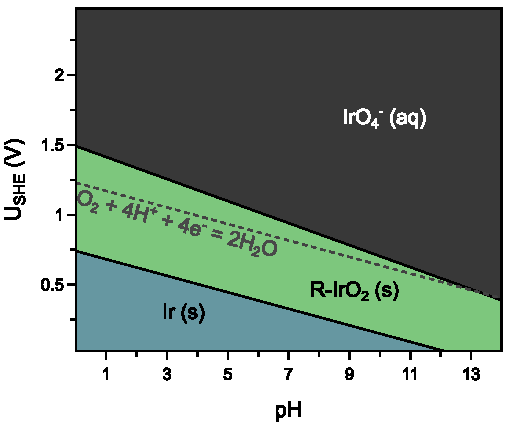
\includegraphics
{02_figures/SI_figures/00_master__bulk-pourbaix__v5.pdf}}
\caption{\label{fig:bulk_pourbaix_wo_alpha}
%
Bulk Pourbaix diagram of the \ce{Ir}-\ce{H2O} system as a function of the applied potential and pH.
%
The diagram was constructed using all of the same species as Figure \ref{fig:bulk_pourbaix} with the exception of any \IrOthree phase, including the globally stable \aIrOthree.
}
\end{figure*}
% __| =====================================================
% =========================================================


% %%%%%%%%%%%%%%%%%%%%%%%%%%%%%%%%%%%%%%%%%%%%%%%%%%%%%%%%%
\subsection{Computational methodology for bulk and surface stability, and OER thermodynamics}
% %%%%%%%%%%%%%%%%%%%%%%%%%%%%%%%%%%%%%%%%%%%%%%%%%%%%%%%%%
%
% %%%%%%%%%%%%%%%%%%%%%%%%%%%%%%%%%%%%%%%%%%%%%%%%%%%%%%%%%
% | - OER Thermodynamic Methodology
%
Here we will outline the procedure used to carry out OER simulations on the various slabs of \IrOtwo and \IrOthree.
%
The procedure was as follows:
%
Stable stoichiometric terminations were cut from the bulk by cleaving along the Miller indices with the highest calculated diffraction peaks, corresponding to planes with higher density of atoms.
%
The location of the cutting plane was further chosen to minimize number of severed bonds in the terminating octahedra.
%
Next, electrochemical surface coverage was predicted via a surface Pourbaix analysis,~\cite{Lu2017}
which is based on relative free energies of OH* and O* coverages as described in the next section.
%
This elucidates the coverage under operating conditions ($>$\num{1.23} \VRHE) for each slab.
%
% COMBAK
Finally, we conducted a thermodynamic limiting potential analysis of the acidic OER single-site associative pathway.
~\cite{Rossmeisl2007,Man2011,Friebel2015,Seitz2016,Strickler2019}
%
The method to construct the OER volcano plot, limiting potentials and free-energy corrections is identical to our most recent works on \IrOtwo systems~\cite{Strickler2019,Lee2020}.
% __|


% %%%%%%%%%%%%%%%%%%%%%%%%%%%%%%%%%%%%%%%%%%%%%%%%%%%%%%%%%
\subsection{Computational methodology for surface energy Pourbaix diagrams}
% %%%%%%%%%%%%%%%%%%%%%%%%%%%%%%%%%%%%%%%%%%%%%%%%%%%%%%%%%
%
% %%%%%%%%%%%%%%%%%%%%%%%%%%%%%%%%%%%%%%%%%%%%%%%%%%%%%%%%%
% | - Surface Energy Pourbaix Methodology
%
Surface energy Pourbaix plots were constructed by calculating the surface energy of symmetric slabs under standard conditions (\si{\volt}\num{=0} and pH\num{=0}) and then utilizing the computational hydrogen electrode (CHE) to compute the potential dependence of the surfaces.
%
Surface energy calculations were performed for various facets for slabs of increasing thickness.
%
% TODO Insert reference for surface E calcs
The bulk energy was then extracted by fitting the total energy of the slabs against the number of layers as explained in Fiorentini \latin{et. al}~\cite{Boettger1998}.
%
This was done to avoid common issues of surface energy divergence associated with using a separate bulk energy calculation.
%
The sensitivity of a given slab to an applied bias is dependent on the composition of the surface,
in particular, the effect of coverage of electrolyte species which can deposit oxygen, hydrogen, and hydroxide species on the surface layers.
%
These additional non-stoichiometric \ce{O} and \ce{H} atoms are not referenced to the atoms in the slab,
but are instead referenced to the computational hydrogen electrode and water-splitting reaction as is commonly done for surface Pourbaix diagrams~\cite{Lu2017}.
%
As such our surface energies,
at \si{\volt}\num{=0} and pH\num{=0},
correspond not only to the energy it takes to cleave a surface (regular surface energy),
but also with the energy associated with removing oxygen and hydrogen atoms from their \ce{H_{2}O} and \ce{H_{2}} references and adding them to the slab's surface.
% __|

% %%%%%%%%%%%%%%%%%%%%%%%%%%%%%%%%%%%%%%%%%%%%%%%%%%%%%%%%%
\subsection{Scaling relations between OER intermediates}
% %%%%%%%%%%%%%%%%%%%%%%%%%%%%%%%%%%%%%%%%%%%%%%%%%%%%%%%%%
%
% %%%%%%%%%%%%%%%%%%%%%%%%%%%%%%%%%%%%%%%%%%%%%%%%%%%%%%%%%
% %%%%%%%%%%%%%%%%%%%%%%%%%%%%%%%%%%%%%%%%%%%%%%%%%%%%%%%%%
% | - OER Scaling Relations

% %%%%%%%%%%%%%%%%%%%%%%%%%%%%%%%%%%%%%%%%%%%%%%%%%%%%%%%%%
% | - Highlight IrO3 is weaker binding
%
% __|
% %%%%%%%%%%%%%%%%%%%%%%%%%%%%%%%%%%%%%%%%%%%%%%%%%%%%%%%%%
% | - PARAGRAPH BODY
%
Figure~\ref{fig:scaling_relations} shows the scaling relations between the adsorption free energies of the OER intermediate species for the studied \IrOx slabs.
%
It can be seen clearly that the data points corresponding to the three \IrOthree polymorphs are roughly \SI{1}{\electronvolt} weaker binding than the \rIrOtwo points.
%
This weaker binding of the \IrOthree stoichiometry is responsible for the observed improvement in theoretical activity.
%
The weaker binding of \IrOthree relative to \IrOtwo is easily rationalized in terms of the formal oxidation state of the Ir atoms.
%
\IrOthree has a $6+$ oxidation state compared to $4+$ for \IrOtwo due to the larger number of oxygens per formula unit.
%
The propensity for \IrOthree to adsorb oxygenated OER intermediates is lessened because it is essentially oversaturated in oxygen compared to \IrOtwo.
%
Thus the stoichiometry of an oxide is a straightforward way to modulate the oxidation state and binding trends in a material system.
% __|
%%%%%%%%%%%%%%%%%%%%%%%%%%%%%%%%%%%%%%%%%%%%%%%%%%%%%%%%%%%


% %%%%%%%%%%%%%%%%%%%%%%%%%%%%%%%%%%%%%%%%%%%%%%%%%%%%%%%%%
% | -
%
% __|
% %%%%%%%%%%%%%%%%%%%%%%%%%%%%%%%%%%%%%%%%%%%%%%%%%%%%%%%%%
% | - PARAGRAPH BODY
%
The scaling relations in our \IrOx data set exhibits deviations from standard scaling relations~\cite{Man2011}.
%
In particular, the adsorption energy of *OOH (\DGOOH) in our dataset is stabilized relative to standard scaling relations.
%
We have
\DGOOH$=1.16$\DGOH$+2.8 eV$ while standard scaling is
\DGOOH$=$\DGOH$+3.2 eV$.
%
Fixing the slope in our data fit to \num{1} to compare the intercepts results in an intercept of \num{2.99} eV for our dataset,
0.2 eV more stable than standard scaling.
%
This stabilization of *OOH relative to *OH is beneficial to the activity and is the reason that the fit volcano (grey) in Figure \ref{fig:oer_volcano}b has a higher activity than the volcano constructed from standard scaling (black).
%
It should be noted that quantity of OER data we are fitting to is relatively small,
and so our confidence in our fit is not robust.
%
Thus it is unclear whether \IrOthree surfaces truly exhibit enhanced scaling or whether the observed enhancement is due to numerical noise.
%
Further studies exploring the OER binding trends in a larger number of \IrOtwo and \IrOthree systems are needed to address this question.


% The \DGOOH vs.\DGOH relationship is
%
%  close to the universal scaling relations,~\cite{Man2011}
% although
%
% demonstrating that our materials do not break the infamous \DGOOH vs. \DGOH scaling.
% __|
%%%%%%%%%%%%%%%%%%%%%%%%%%%%%%%%%%%%%%%%%%%%%%%%%%%%%%%%%%%




% __|


% =========================================================
% FIGURE ==================================================
% =========================================================
% | - Figure | OER Scaling Relations
\begin{figure*}[!htb]
\centering
\makebox[\textwidth][c]{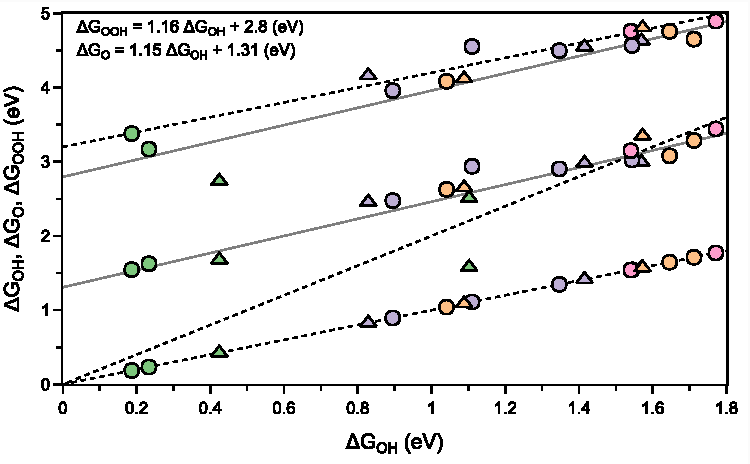
\includegraphics
{02_figures/SI_figures/00_master__oer_scaling__main_v4.pdf}}
\caption{\label{fig:scaling_relations}
%
Relationship between the adsorption free energies of the three key OER intermediates (*OH, *O, *OOH), with \DGOH chosen as the dependent variable.
%
Best fit lines (solid grey) are provided for \DGOOH vs. \DGOH and \DGO vs. \DGOH.
%
The meaning of symbols is identical to Figure~\ref{fig:oer_volcano}, main text.
%
The standard ``universal scaling relations'' for \DGOOH vs. \DGOH and \DGO vs. \DGOH are shown (black dotted lines) to emphasize our deviation from the traditionally reported scaling fits.
%
The \DGOH line is shown as guide to eye.
}
\end{figure*}
% __| =====================================================
% =========================================================


% %%%%%%%%%%%%%%%%%%%%%%%%%%%%%%%%%%%%%%%%%%%%%%%%%%%%%%%%%
\subsection{Tabulated OER adsorption energies}
% %%%%%%%%%%%%%%%%%%%%%%%%%%%%%%%%%%%%%%%%%%%%%%%%%%%%%%%%%
%
% %%%%%%%%%%%%%%%%%%%%%%%%%%%%%%%%%%%%%%%%%%%%%%%%%%%%%%%%%
% %%%%%%%%%%%%%%%%%%%%%%%%%%%%%%%%%%%%%%%%%%%%%%%%%%%%%%%%%
% | - Table of OER energetics


% %%%%%%%%%%%%%%%%%%%%%%%%%%%%%%%%%%%%%%%%%%%%%%%%%%%%%%%%%
% | -
%
% __|
% %%%%%%%%%%%%%%%%%%%%%%%%%%%%%%%%%%%%%%%%%%%%%%%%%%%%%%%%%
% | - PARAGRAPH BODY
%
Table \ref{table:oer_data} contains the adsorbate binding energetics for the intermediates of the OER
oxygen evolution reaction (*O, *OOH, *OH).
% __|
%%%%%%%%%%%%%%%%%%%%%%%%%%%%%%%%%%%%%%%%%%%%%%%%%%%%%%%%%%%


% __|


% =========================================================
% TABLE ===================================================
% =========================================================
% | - Table | OER energetics
\newpage  % request a new page.
\begin{landscape}
\renewcommand{\arraystretch}{1.5} % <--------------
\begin{table}
\resizebox{\linewidth}{!}{%
\centering
\caption{\label{table:oer_data}
%
OER adsorption energies for slabs of \IrOtwo and \IrOthree polymorphs studied here.
%
Included quantities are electronic adsorption energies
($\Delta E_{O_{x}H_{y}}$),
adsorption free energies
($\Delta G_{O_{x}H_{y}}$),
as well as the \DGOmOH{} OER descriptor.
%
Coverage indicates the electrochemical coverage of either *O or *OH species.
% %
The limiting potential and corresponding overpotential ($\eta$) as well as the rate determining step (RDS) for the OER mechanism are shown.
%
All optimized slab models and corresponding DFT energies are freely available under the ``FloresActive2020''~\cite{upload_CatHub} dataset at Catalysis-hub.org~\cite{Winther2019}.
}
\begin{tabular}{lllcccccccccc}
\toprule
                Bulk Sys. &    Facet &    Coverage & $\Delta E_{*OH}$ & $\Delta E_{*O}$ & $\Delta E_{*OOH}$ & $\Delta G_{*OH}$ & $\Delta G_{*O}$ & $\Delta G_{*OOH}$ & $\Delta G_{*O}-\Delta G_{*OH}$ & Lim. Pot. & $\eta$ &                                                                    RDS \\
                        - &        - &           - &             (eV) &            (eV) &              (eV) &             (eV) &            (eV) &              (eV) &                           (eV) &       (V) &    (V) &                                                                      - \\
\midrule
      $R{\text -}IrO_{2}$ &    (100) &         *OH &            0.130 &           1.634 &             2.362 &            0.424 &           1.678 &             2.738 &                          1.254 &     2.182 &  0.952 &              $*OOH \rightarrow * \phantom{T} \phantom{T} \phantom{T} $ \\
      $R{\text -}IrO_{2}$ &    (100) &          *O &           -0.061 &           1.582 &             2.793 &            0.234 &           1.626 &             3.170 &                          1.392 &     1.750 &  0.520 &              $*OOH \rightarrow * \phantom{T} \phantom{T} \phantom{T} $ \\
      $R{\text -}IrO_{2}$ &    (110) &         *OH &            0.807 &           1.535 &             2.133 &            1.102 &           1.579 &             2.509 &                          0.477 &     2.411 &  1.181 &              $*OOH \rightarrow * \phantom{T} \phantom{T} \phantom{T} $ \\
      $R{\text -}IrO_{2}$ &    (110) &          *O &           -0.108 &           1.503 &             3.004 &            0.187 &           1.547 &             3.380 &                          1.360 &     1.833 &  0.603 &                         $*O \phantom{T} \phantom{T}  \rightarrow *OOH$ \\
 $\alpha{\text -}IrO_{3}$ &    (100) &         *OH &            1.275 &           2.950 &             4.254 &            1.569 &           2.994 &             4.630 &                          1.424 &     1.636 &  0.406 &                         $*O \phantom{T} \phantom{T}  \rightarrow *OOH$ \\
 $\alpha{\text -}IrO_{3}$ &    (100) &          *O &            1.249 &           2.980 &             4.191 &            1.544 &           3.024 &             4.567 &                          1.480 &     1.544 &  0.314 &  $* \phantom{T} \phantom{T} \phantom{T}  \rightarrow *OH \phantom{T} $ \\
 $\alpha{\text -}IrO_{3}$ &    (110) &         *OH &            0.534 &           2.414 &             3.786 &            0.828 &           2.458 &             4.163 &                          1.629 &     1.705 &  0.475 &                         $*O \phantom{T} \phantom{T}  \rightarrow *OOH$ \\
 $\alpha{\text -}IrO_{3}$ &    (110) &          *O &            0.600 &           2.432 &             3.582 &            0.895 &           2.476 &             3.959 &                          1.581 &     1.581 &  0.351 &              $*OH \phantom{T} \rightarrow *O \phantom{T} \phantom{T} $ \\
 $\alpha{\text -}IrO_{3}$ &    (111) &          *O &            0.815 &           2.894 &             4.177 &            1.110 &           2.938 &             4.554 &                          1.828 &     1.828 &  0.598 &              $*OH \phantom{T} \rightarrow *O \phantom{T} \phantom{T} $ \\
 $\alpha{\text -}IrO_{3}$ &    (211) &         *OH &            1.120 &           2.937 &             4.173 &            1.415 &           2.981 &             4.549 &                          1.566 &     1.568 &  0.338 &                         $*O \phantom{T} \phantom{T}  \rightarrow *OOH$ \\
 $\alpha{\text -}IrO_{3}$ &    (211) &          *O &            1.052 &           2.860 &             4.122 &            1.347 &           2.904 &             4.499 &                          1.558 &     1.594 &  0.364 &                         $*O \phantom{T} \phantom{T}  \rightarrow *OOH$ \\
  $\beta{\text -}IrO_{3}$ &  (010)-A &          *O &            1.246 &           3.105 &             4.383 &            1.541 &           3.149 &             4.759 &                          1.609 &     1.610 &  0.380 &                         $*O \phantom{T} \phantom{T}  \rightarrow *OOH$ \\
  $\beta{\text -}IrO_{3}$ &  (010)-B &          *O &            1.477 &           3.399 &             4.519 &            1.771 &           3.443 &             4.896 &                          1.672 &     1.771 &  0.541 &  $* \phantom{T} \phantom{T} \phantom{T}  \rightarrow *OH \phantom{T} $ \\
      $R{\text -}IrO_{3}$ &    (100) &         *OH &            1.278 &           3.304 &             4.431 &            1.572 &           3.348 &             4.807 &                          1.776 &     1.776 &  0.546 &              $*OH \phantom{T} \rightarrow *O \phantom{T} \phantom{T} $ \\
      $R{\text -}IrO_{3}$ &    (100) &          *O &            1.351 &           3.036 &             4.381 &            1.646 &           3.080 &             4.758 &                          1.435 &     1.677 &  0.447 &                         $*O \phantom{T} \phantom{T}  \rightarrow *OOH$ \\
      $R{\text -}IrO_{3}$ &    (100) &  *O-partial &            1.417 &           3.243 &             4.275 &            1.712 &           3.287 &             4.652 &                          1.575 &     1.712 &  0.482 &  $* \phantom{T} \phantom{T} \phantom{T}  \rightarrow *OH \phantom{T} $ \\
      $R{\text -}IrO_{3}$ &    (110) &         *OH &            0.794 &           2.607 &             3.744 &            1.088 &           2.651 &             4.121 &                          1.563 &     1.563 &  0.333 &              $*OH \phantom{T} \rightarrow *O \phantom{T} \phantom{T} $ \\
      $R{\text -}IrO_{3}$ &    (110) &          *O &            0.746 &           2.583 &             3.708 &            1.041 &           2.627 &             4.084 &                          1.586 &     1.586 &  0.356 &              $*OH \phantom{T} \rightarrow *O \phantom{T} \phantom{T} $ \\
\bottomrule
\end{tabular}

}
\end{table}

\end{landscape}
% __| =====================================================
% =========================================================















% | - WORK IN PROGRESS

% %%%%%%%%%%%%%%%%%%%%%%%%%%%%%%%%%%%%%%%%%%%%%%%%%%%%%%%%%
% %%%%%%%%%%%%%%%%%%%%%%%%%%%%%%%%%%%%%%%%%%%%%%%%%%%%%%%%%
% %%%%%%%%%%%%%%%%%%%%%%%%%%%%%%%%%%%%%%%%%%%%%%%%%%%%%%%%%
% %%%%%%%%%%%%%%%%%%%%%%%%%%%%%%%%%%%%%%%%%%%%%%%%%%%%%%%%%
% %%%%%%%%%%%%%%%%%%%%%%%%%%%%%%%%%%%%%%%%%%%%%%%%%%%%%%%%%
% %%%%%%%%%%%%%%%%%%%%%%%%%%%%%%%%%%%%%%%%%%%%%%%%%%%%%%%%%
% %%%%%%%%%%%%%%%%%%%%%%%%%%%%%%%%%%%%%%%%%%%%%%%%%%%%%%%%%
% %%%%%%%%%%%%%%%%%%%%%%%%%%%%%%%%%%%%%%%%%%%%%%%%%%%%%%%%%

% % %%%%%%%%%%%%%%%%%%%%%%%%%%%%%%%%%%%%%%%%%%%%%%%%%%%%%%%%%
% \subsection{Bulk Systems}  % %%%%%%%%%%%%%%%%%%%%%%%%%%%%%%
% % %%%%%%%%%%%%%%%%%%%%%%%%%%%%%%%%%%%%%%%%%%%%%%%%%%%%%%%%%
% %
% % %%%%%%%%%%%%%%%%%%%%%%%%%%%%%%%%%%%%%%%%%%%%%%%%%%%%%%%%%
% % %%%%%%%%%%%%%%%%%%%%%%%%%%%%%%%%%%%%%%%%%%%%%%%%%%%%%%%%%
% % | - Bulk Systems
%
%
% % %%%%%%%%%%%%%%%%%%%%%%%%%%%%%%%%%%%%%%%%%%%%%%%%%%%%%%%%%
% % | -
% %
% % __|
% % %%%%%%%%%%%%%%%%%%%%%%%%%%%%%%%%%%%%%%%%%%%%%%%%%%%%%%%%%
% % | - PARAGRAPH BODY
% % Formation energies of 4 polymorphs
% % __|
% %%%%%%%%%%%%%%%%%%%%%%%%%%%%%%%%%%%%%%%%%%%%%%%%%%%%%%%%%%%
%
%
% % __|

% %%%%%%%%%%%%%%%%%%%%%%%%%%%%%%%%%%%%%%%%%%%%%%%%%%%%%%%%%
% %%%%%%%%%%%%%%%%%%%%%%%%%%%%%%%%%%%%%%%%%%%%%%%%%%%%%%%%%
% %%%%%%%%%%%%%%%%%%%%%%%%%%%%%%%%%%%%%%%%%%%%%%%%%%%%%%%%%
% %%%%%%%%%%%%%%%%%%%%%%%%%%%%%%%%%%%%%%%%%%%%%%%%%%%%%%%%%
% %%%%%%%%%%%%%%%%%%%%%%%%%%%%%%%%%%%%%%%%%%%%%%%%%%%%%%%%%
% %%%%%%%%%%%%%%%%%%%%%%%%%%%%%%%%%%%%%%%%%%%%%%%%%%%%%%%%%
% %%%%%%%%%%%%%%%%%%%%%%%%%%%%%%%%%%%%%%%%%%%%%%%%%%%%%%%%%
% %%%%%%%%%%%%%%%%%%%%%%%%%%%%%%%%%%%%%%%%%%%%%%%%%%%%%%%%%


% __|
